\setAuthor{Mihkel Kree}
\setRound{lahtine}
\setYear{2013}
\setNumber{G 8}
\setDifficulty{7}
\setTopic{Staatika}

\prob{Niidirull}
\begin{wrapfigure}[6]{r}{3cm}
\vspace{-15pt}
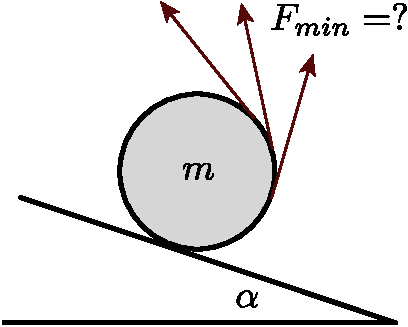
\includegraphics[width=\linewidth]{2013-lahg-08-joonis_niidirull-crop}
\end{wrapfigure}

Silinder massiga $m$, millele on keritud õhuke niit, asetatakse kaldpinnale nurgaga $\alpha$.
Millise minimaalse jõuga $F\idx{min}$ tuleb nöörist hoida, et silinder paigale
jääks (vt joonist)? Hõõrdetegur pinna ja silindri vahel on nii suur, et
libisemist ei toimu.

\hint
Silindril peab kehtima nii jõudude kui ka jõumomentide tasakaal. Jõumomentide tasakaalu on mugav vaadelda telje suhtes, mis läbib toetuspunkti, sest siis on hõõrdejõu ja toereaktsiooni jõuõlg \num{0}.

\solu
Vaatleme silindrile mõjuvate jõumomentide tasakaalu telje suhtes, mis läbib toetuspunkti. Pinna toereaktsiooni ja hõõrdejõu vektorid läbivad toetuspunkti, mistõttu need jõumomenti ei tekita. Jõumomendi tekitavad kaks jõudu: silindri keskele rakendatud raskusjõud $mg$ ja nööri tõmbejõud $F$. Arvutades lihtsast kolmnurgast raskusjõu õla, saame jõumomendiks $\tau=mgr\sin\alpha$. Tasakaalu korral tekitab tõmbejõud $F$ sama suure, kuid vastassuunalise jõumomendi $-\tau$. Minimaalsele jõule peab vastama maksimaalne jõuõlg. Veendume, et kui jõud $F$ rakendada toetuspunktist diametraalselt vastas olevasse punkti, saame maksimaalse õla $2r$, millele vastab minimaalne tõmbejõud
\[F\idx{min}=\frac{\tau}{2r}=\frac{mg\sin\alpha}{2}.\]

\probeng{Thread roll}
\begin{wrapfigure}[6]{r}{3cm}
\vspace{-15pt}
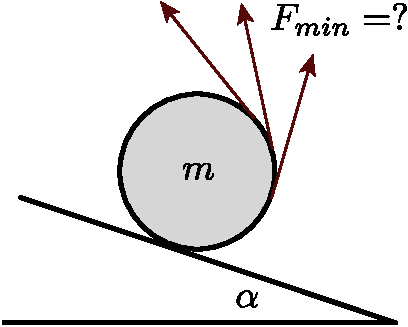
\includegraphics[width=\linewidth]{2013-lahg-08-joonis_niidirull-crop}
\end{wrapfigure}
A cylinder of mass $m$ has a thin thread winded over it and it is placed on an inclined surface with an inclination angle of $\alpha$. What is the required minimal force $F\idx{min}$ to hold the thread so that the cylinder would stay still (see figure)? The coefficient of friction between the surface and the cylinder is so big that there is no sliding.

\hinteng
Both the force and torque balance has to apply to the cylinder. The torque balance is convenient to observe with respect to the axis that goes through the support point because then the torque arm of friction and normal force is 0.

\solueng
Let us observe the balance of the torques applied to the cylinder with respect to the axis that goes through the support point. The vectors of the surface’s normal force and friction go through the support point which is why they do not create a torque. A torque is created by two forces: the gravity force $mg$ applied to the cylinder’s center and the thread’s pulling force $F$. Calculating the gravity force’s arm from a simple triangle we get the torque to be $\tau=mgr\sin\alpha$. In the case of equilibrium the pulling force $F$ creates a torque $-\tau$ that is as big but has the opposite direction. The minimal force has to correspond to the maximal force arm. Let us make sure that if the force $F$ was applied to a point diametrically opposite to the support point then we get the maximal arm $2r$ that has a corresponding minimal pulling force
\[F\idx{min}=\frac{\tau}{2r}=\frac{mg\sin\alpha}{2}.\]
\probend